\RequirePackage[l2tabu,orthodox]{nag}

% TODO: decide if one-sided/two-sided
%\documentclass[headsepline,footsepline,footinclude=false,fontsize=11pt,paper=a4,listof=totoc,bibliography=totoc,BCOR=12mm,DIV=12]{scrbook} % two-sided
\documentclass[headsepline,footsepline,footinclude=false,
oneside,fontsize=11pt,paper=a4,listof=totoc]{scrbook} % one-sided
%,bibliography=totoc
% TODO: change citation style in settings
\PassOptionsToPackage{table,svgnames,dvipsnames}{xcolor}

\usepackage[utf8]{inputenc}
\usepackage[T1]{fontenc}
\usepackage[sc]{mathpazo}
\usepackage[ngerman,american]{babel}
\usepackage[autostyle]{csquotes}
%\usepackage[%
%  backend=biber,
%  url=false,
%  style=alphabetic,
%  maxnames=4,
%  minnames=3,
%  maxbibnames=99,
%  giveninits,
%  uniquename=init]{biblatex} % TODO: adapt citation style
\usepackage{graphicx}
\usepackage{scrhack} % necessary for listings package
\usepackage{listings}
\usepackage{lstautogobble}
\usepackage{tikz}
\usepackage{pgfplots}
\usepackage{pgfplotstable}
\usepackage{booktabs}
\usepackage[final]{microtype}
\usepackage{caption}
\usepackage[hidelinks]{hyperref} % hidelinks removes colored boxes around references and links

%\bibliography{bibliography}

\setkomafont{disposition}{\normalfont\bfseries} % use serif font for headings
\linespread{1.05} % adjust line spread for mathpazo font

% Add table of contents to PDF bookmarks
\BeforeTOCHead[toc]{{\cleardoublepage\pdfbookmark[0]{\contentsname}{toc}}}

% Define TUM corporate design colors
% Taken from http://portal.mytum.de/corporatedesign/index_print/vorlagen/index_farben
\definecolor{TUMBlue}{HTML}{0065BD}
\definecolor{TUMSecondaryBlue}{HTML}{005293}
\definecolor{TUMSecondaryBlue2}{HTML}{003359}
\definecolor{TUMBlack}{HTML}{000000}
\definecolor{TUMWhite}{HTML}{FFFFFF}
\definecolor{TUMDarkGray}{HTML}{333333}
\definecolor{TUMGray}{HTML}{808080}
\definecolor{TUMLightGray}{HTML}{CCCCC6}
\definecolor{TUMAccentGray}{HTML}{DAD7CB}
\definecolor{TUMAccentOrange}{HTML}{E37222}
\definecolor{TUMAccentGreen}{HTML}{A2AD00}
\definecolor{TUMAccentLightBlue}{HTML}{98C6EA}
\definecolor{TUMAccentBlue}{HTML}{64A0C8}

% Settings for pgfplots
\pgfplotsset{compat=newest}
\pgfplotsset{
  % For available color names, see http://www.latextemplates.com/svgnames-colors
  cycle list={TUMBlue\\TUMAccentOrange\\TUMAccentGreen\\TUMSecondaryBlue2\\TUMDarkGray\\},
}

% Settings for lstlistings
\lstset{%
  basicstyle=\ttfamily,
  columns=fullflexible,
  autogobble,
  keywordstyle=\bfseries\color{TUMBlue},
  stringstyle=\color{TUMAccentGreen}
}


% TODO: change thesis information
\newcommand*{\getUniversity}{Technische Universität München}
\newcommand*{\getFaculty}{Department of Informatics}
\newcommand*{\getTitle}{Time and Space Discretization for One Dimensional PDEs with Application to Climate and Weather Simulations}
\newcommand*{\getTitleGer}{Zeitliche und räumliche Diskretisierung für eindimensionale PDGLs mit Anwendung in Klima- und Wettersimulationen}
\newcommand*{\getAuthor}{Linus Hein}
\newcommand*{\getDoctype}{Bachelor's Thesis in Informatics}
\newcommand*{\getSupervisor}{Prof. Martin Schulz}
\newcommand*{\getAdvisor}{Martin Schreiber}
\newcommand*{\getSubmissionDate}{15.08.2019}
\newcommand*{\getSubmissionLocation}{Munich}

\usepackage{amsmath}
\usepackage{makecell}
\usepackage{tabu}

%\usepackage{biblatex}
%\addbibresource{bibliography.bib}
\bibliographystyle{unsrt}

\begin{document}


% Set page numbering to avoid "destination with the same identifier has been already used" warning for cover page.
% (see https://en.wikibooks.org/wiki/LaTeX/Hyperlinks#Problems_with_Links_and_Pages).
\pagenumbering{alph}
\begin{titlepage}
  % HACK for two-sided documents: ignore binding correction for cover page.
  % Adapted from Markus Kohm's KOMA-Script titlepage=firstiscover handling.
  % See http://mirrors.ctan.org/macros/latex/contrib/koma-script/scrkernel-title.dtx,
  % \maketitle macro.
  \oddsidemargin=\evensidemargin\relax
  \textwidth=\dimexpr\paperwidth-2\evensidemargin-2in\relax
  \hsize=\textwidth\relax

  \centering

  \IfFileExists{logos/tum.pdf}{%
    \includegraphics[height=20mm]{logos/tum.pdf}
  }{%
    \vspace*{20mm}
  }

  \vspace{5mm}
  {\huge\MakeUppercase{\getFaculty{}}}\\

  \vspace{5mm}
  {\large\MakeUppercase{\getUniversity{}}}\\

  \vspace{20mm}
  {\Large \getDoctype{}}

  \vspace{15mm}
  {\huge\bfseries \getTitle{}}

  \vspace{15mm}
  {\LARGE \getAuthor{}}

  \IfFileExists{logos/faculty.pdf}{%
    \vfill{}
    \includegraphics[height=20mm]{logos/faculty.pdf}
  }{}
\end{titlepage}


\frontmatter{}

\begin{titlepage}
  \centering

  \IfFileExists{logos/tum.pdf}{%
    \includegraphics[height=20mm]{logos/tum.pdf}
  }{%
    \vspace*{20mm}
  }

  \vspace{5mm}
  {\huge\MakeUppercase{\getFaculty{}}}\\

  \vspace{5mm}
  {\large\MakeUppercase{\getUniversity{}}}\\

  \vspace{20mm}
  {\Large \getDoctype{}}

  \vspace{15mm}
  {\huge\bfseries \getTitle{}}

  \vspace{10mm}
  {\huge\bfseries \foreignlanguage{ngerman}{\getTitleGer{}}}

  \vspace{15mm}
  \begin{tabular}{l l}
    Author:          & \getAuthor{} \\
    Supervisor:      & \getSupervisor{} \\
    Advisor:         & \getAdvisor{} \\
    Submission Date: & \getSubmissionDate{} \\
  \end{tabular}

  \IfFileExists{logos/faculty.pdf}{%
    \vfill{}
    \includegraphics[height=20mm]{logos/faculty.pdf}
  }{}
\end{titlepage}

\thispagestyle{empty}
\vspace*{0.8\textheight}
\noindent
I confirm that this \MakeLowercase{\getDoctype{}} is my own work and I have documented all sources and material used.

\vspace{15mm}
\noindent
\getSubmissionLocation{}, \getSubmissionDate{} \hspace{50mm} \getAuthor{}

\cleardoublepage{}

\addcontentsline{toc}{chapter}{Acknowledgments}
\thispagestyle{empty}

\vspace*{20mm}

\begin{center}
{\usekomafont{section} Acknowledgments}
\end{center}

\vspace{10mm}

%TODO: Acknowledgments
\noindent
I want to thank my advisor, Dr. Martin Schreiber, for giving me helpful pointers whenever I thought I was at a dead end.
I also want to thank my supervisor, Prof. Dr. Schulz, for allowing me to pursue this subject, even though it is only tangentially related to his main area of research.\\
Finally, I want to thank my family and friends who have always supported me throughout my studies.

\cleardoublepage{}

\chapter{\abstractname}
Weather and climate models based on the Navier Stokes Equations often employ the hydrostatic assumption whereby one assumes the atmosphere to be in vertical equilibrium between gravity and vertical air pressure.
As this assumption affects the simulated physical effects, in this thesis, we relax the hydrostatic assumption, and specifically study the vertical dimension.
To this end, we present a tested, modular and flexible prototyping implementation in Python 3 which provides complete access to integration methods and discretization.
%We then validate the implementation using a suite of test cases.
\microtypesetup{protrusion=false}
\tableofcontents{}
\microtypesetup{protrusion=true}

\mainmatter{}

% !TeX root = ../main.tex
% Add the above to each chapter to make compiling the PDF easier in some editors.

\chapter{Introduction}\label{chapter:introduction}

At one point or another, most parts of applied physics and engineering make use of partial differential equations (PDEs), which are equations describing how the state of a system will evolve.
And while a small subset of these PDEs can be solved analytically, i.e. it is possible to write down a mathematical formula that solves the PDE and thus describes the system in any state, it is more common to come across PDEs which are not solvable in such a way.
Instead it becomes necessary to approximate solutions to such PDEs numerically.
Generally this process can be split up into four steps:
\begin{enumerate}
\item \emph{Modeling}: finding a system of PDEs that describe a system
\item \emph{Approximating}: simplifying the system of PDEs by making assumptions about the system (e.g. small angle approximation for a pendulum system)
\item \emph{Space Discretization}: if the system contains scalar- or vector-fields, choosing the locations at which to store the values of each individual field
\item \emph{Time Discretization}: choosing an integration method
\end{enumerate}
Each of these four steps introduce different trade-offs between computational efficiency and errors.
This thesis will go through all of these four steps by applying them to a strongly simplified model of weather.
More specifically this thesis will only look into the vertical part of weather simulation using the Navier-Stokes equations.
The vertical part is viewed in isolation, because current weather simulation tools often split up the vertical and horizontal part of simulation by alternating between simulating horizontal and vertical effects. [TODO: find source]
After applying the four steps to the system, the errors introduced by the possible choices in each of the steps will be analyzed.
To this end, the numerical approximation was implemented using Python 3.
The software architecture behind this implementation will be described in section \ref{chapter:software}.
\chapter{Navier Stokes Equations}\label{chapter:introduction}
Navier Stokes Equations\\
explanation of terms

\section{Assumptions, Simplifications, and Modifications}
\subsection{Alternative Coordinate Systems}
\subsection{Boundary Conditions}

\section{Grid Discretizations}

\chapter{Discretization}\label{chapter:discretization}
Having discussed the NSE and the different kinds of rearrangements and simplifications, we completed the first two steps of \emph{modeling} and \emph{approximating}.
Next, we address the problem of simulating the NSE on computers with finite memory and computational capacity.
To this end, we must discretize all the continuous spatial and temporal terms in the NSE, in order to make the memory and time required for computation finite.
These discretizations account for Step 3 (\emph{Space Discretization}) and Step 4 (\emph{Time Discretization}) of solving a PDE numerically.

The meaning of discretization can be seen by looking at one of the equations to be discretized:
\begin{align*}
\frac{\partial w}{\partial t} &= -g\left(1 - \frac{\partial p}{\partial s}\left(\frac{\partial \pi}{\partial s}\right)^{-1}\right)
\end{align*}
First, spatial derivatives and other spatial differential operators like $\frac{\partial p}{\partial s}$ must be discretized, i.e. they must be approximated.
This must be done using a finite number of samples of $p$ around the point where the derivative is to be calculated.

Second, $w$ and $p$ must be discretized themselves.
In the real world these are continuous in space.
However, when computing, we can only represent them with a finite number of samples.
Usually, every variable in a differential equation is assigned to a grid, and at every node of that grid a measurement of the variable is stored.

Third, we must discretize the time variable in $\frac{\partial w}{\partial t}$.
To be more specific, we need to reverse the time derivative, i.e. integrate it, in order to gain the real value of $w$ from the diagnostic equation for $\frac{\partial w}{\partial t}$.

In summary, we assume the state of the system at time $t$ to be represented by a number of variables stored in the nodes of a grid.
Next we evaluate the value of the differential equation at those grid nodes.
We approximate any spatial derivative required for this through its respective discrete spatial derivative.
For these discrete spacial derivatives we only make use of the variable values at the grid points.
To approximate the state of the system at some other discrete time $t+\Delta t$, we then input the value of the differential equation to an integrator which reverses the time derivative.

\subsubsection{Overview}
In Section~\ref{section:diff_op} we address the discretization of differential operators.
In Section~\ref{sec:grid_discretization} we discuss the important issue of discretization of prognostic variables onto a regular grid.
In Section~\ref{sec:integrators} we present the integration operators which we implemented for this thesis.

\section{Discretization of Differential Operators}\label{section:diff_op}
In this section we present two methods for approximating spatial derivatives using only samples at discrete spatial locations.
The first method is called finite differences and approximates the derivative at a location by only looking at samples close to that location.
While not always the most accurate, this method makes no assumptions\footnote{except for sufficient differentiability} about the function it is taking the derivative of.

The second method (sometimes called spectral) takes a detour to the frequency domain to approximate the derivative.
While this method is highly accurate when applicable, it assumes the boundary conditions to be periodic.
This is not the case for the vertical dimension of weather simulation, hence we cannot employ this method for simulating the vertical dimension of the NSE.
We present it nonetheless, because it plays a central role for numerical weather prediction in the horizontal dimension.

\subsection{Finite Differences}
In order to derive the commonly known (e.g. refer to~\cite{smith1985numerical}) finite difference operators, we must introduce the Taylor Series.
It approximates a function around a given point with polynomials and spatial derivatives as follows.

Let $f:\mathbb{R}\times\mathbb{R}^q\rightarrow \mathbb{R}$ be a function which we want to develop along its first argument $x$.
All other inputs $\boldsymbol{v}$ are held constant.
Employing the Landau notation, and with $\mathcal{O}(\Delta x ^{n+1})$ being the error of the approximation, the following holds:
\begin{equation}
f(x+\Delta x,v) = \sum_{k=0}^{n}\frac{1}{k!}\cdot\frac{\partial^k f}{\partial x ^k}(x,v)\cdot \Delta x^k + \mathcal{O}(\Delta x ^{n+1})
\end{equation}
Assuming an equidistant grid, i.e. the values of $f(x+k\Delta x,v)$ for $k\in [-l,u] \cap \mathbb{Z}$ are known, this yields a linear equation system of size $l + u + 1 - 1= l + u$ ($-1$ because $k=0$ yields no information).
In the following, we omit the second argument $v$ in the equations.

\begin{align*}
f(x - l \Delta x) &= f(x) + \frac{1}{1!}\cdot\frac{\partial f}{\partial x}(x)\cdot (-l\Delta x)^1 + \frac{1}{2!}\cdot\frac{\partial^2 f}{\partial x^2}(x)\cdot (-l\Delta x)^2 + ... + \mathcal{O}((\Delta x) ^{l+u+1})\\
&...\\
f(x) &= f(x) + \frac{1}{1!}\cdot\frac{\partial f}{\partial x}(x)\cdot (0)^1 + \frac{1}{2!}\cdot\frac{\partial^2 f}{\partial x^2}(x)\cdot (0)^2 + ... + \mathcal{O}((0) ^{l+u+1})= f(x)\\
&...\\
f(x + u \Delta x) &= f(x) + \frac{1}{1!}\cdot\frac{\partial f}{\partial x}(x)\cdot (u\Delta x)^1 + \frac{1}{2!}\cdot\frac{\partial^2 f}{\partial x^2}(x)\cdot (u\Delta x)^2 + ... + \mathcal{O}((\Delta x) ^{l+u+1})\\
\end{align*}
The equation system consists of $l+u$ unknowns, i.e. $\frac{\partial^k f}{\partial x^k}(x,v)$, and $l+u$ equations.
The error of the approximation made by solving for one of the unknowns $\frac{\partial^k f}{\partial x^k}(x,v)$ is $\mathcal{O}((\Delta x) ^{l+u+1-k})$ ($-k$ comes from the fact that the equation must be divided by $\Delta x ^k$ before being solved).
In this thesis we mostly apply the first derivative.
To this end, we mostly use the following four configurations which are also visualized in Fig.~\ref{fig:finite_differences}:

\begin{figure}[!h]
	\makebox[\textwidth]{ 
  		 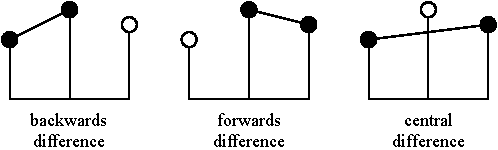
\includegraphics[width=0.9\textwidth]{figures/forwards_backwards_central.pdf}}
    \caption{Visualization of forwards ($l=0,u=1$), backwards ($l=1,u=0$), and central differences ($l=1,u=1$)}
    \label{fig:finite_differences}
\end{figure}

\begin{align*}
l=0,u=1&: \frac{\partial f}{\partial x}(x) = \frac{f(x+\Delta x) - f(x)}{\Delta x} + \mathcal{O}((\Delta x)^{1})\\
l=1,u=0&: \frac{\partial f}{\partial x}(x) = \frac{f(x) - f(x-\Delta x)}{\Delta x} + \mathcal{O}((\Delta x)^{1})\\
l=1,u=1&: \frac{\partial f}{\partial x}(x) = \frac{f(x + \Delta x) - f(x-\Delta x)}{2\Delta x} + \mathcal{O}((\Delta x)^{2})\\
l=2,u=2&: \frac{\partial f}{\partial x}(x) = \frac{f(x-2\Delta x) -8 f(x-\Delta x) + 8 f(x+\Delta x) - f(x+2\Delta x)}{12\Delta x} + \mathcal{O}((\Delta x)^{4})\\
\end{align*}


\subsection{Spectral Methods for Periodic Boundary Conditions}
While finite differences are quite intuitive in their nature, the derivative of a function can also be calculated by spectral methods.
For the method presented here, this requires periodic boundary conditions and entails the usage of the Fourier Transform.
According to Johnson~\cite{johnson2011notes}, the intuition behind this can be seen by assuming that any function on a domain $[0;L]$ can be written as a series:
\begin{align*}
y(x) = \sum_{k=-\infty}^{\infty}Y_k\exp \left(\frac{2\pi i}{L}kx\right)
\end{align*}
Given that all $Y_k$ are known, the derivative $\frac{dy}{dx}$ can be written as a new series:
\begin{align*}
\frac{dy}{dx}(x) = \sum_{k=-\infty}^{\infty}\left(\frac{2\pi i}{L}kY_k\right)\exp \left(\frac{2\pi i}{L}kx\right)
\end{align*}
In this example the coefficients $Y_k$ are the Fourier Transform of $y(x)$, and the coefficients $(\frac{2\pi i}{L}kY_k)$ are the Fourier Transform of the derivative $\frac{dy}{dx}(x)$.
As there is clearly a linear relationship between the Fourier coefficients of the function and the coefficients of its derivative, the derivative of any function can be calculated in three steps:
First, calculating the Fourier coefficients of a function.
Second, modifying the calculated Fourier coefficients appropriately.
Third, calculating the derivative by applying the inverse Fourier Transform on the the modified Fourier coefficients, i.e. by calculating $\frac{dy}{dx}(x)$ from $(\frac{2\pi i}{L}kY_k)$.

Given the fact that computers are not dealing with continuous functions, but only with discrete samples thereof, we must apply the discrete Fourier Transform.
It is commonly calculated by means of the Fast Fourier Transform (FFT).
The derivation of this method can be found in~\cite{johnson2011notes}.
\\

The main advantage of this spectral method is its precision as long as the spatial sampling rate is sufficiently high\footnote{In signal-processing terms the sample frequency must exceed the Nyquist frequency, and in this case the accuracy is only limited by numerical effects, such as machine precision}, as will be seen in the numerical testing done in Section~\ref{sec:numeric_diff_ops}.

However, the downsides to this method are twofold.
First, the method requires boundary conditions to be periodic in order to work, because the FFT assumes periodic boundary conditions.
Second, computing the FFT takes $\mathcal{O}(n\log n)$ which is significantly slower than the $\mathcal{O}(n)$ required for finite difference operators.

We introduced the spectral methods nontheless, because they are common when simulating the horizontal dimension of the weather system on a planetary scale~\cite{coiffier2011fundamentals},\cite{chen1997use},\cite{shuman1989history}.
This is possible because in the horizontal dimension a spherical planet has periodic boundary conditions.
That is, if one were to always travel exactly eastward endlessly, one would end up where one started periodically.
In other words, the endless journey eastward is periodic and so are the boundary conditions of the horizontal system.

\section{Grid Discretizations}\label{sec:grid_discretization}
\begin{figure}[ht]
	\makebox[\textwidth]{ 
  		 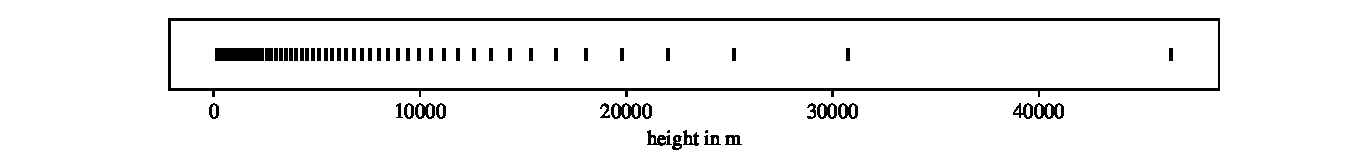
\includegraphics[width=.9\textwidth]{figures/50gridpoints.pdf}}
  	\makebox[\textwidth]{ 
  		 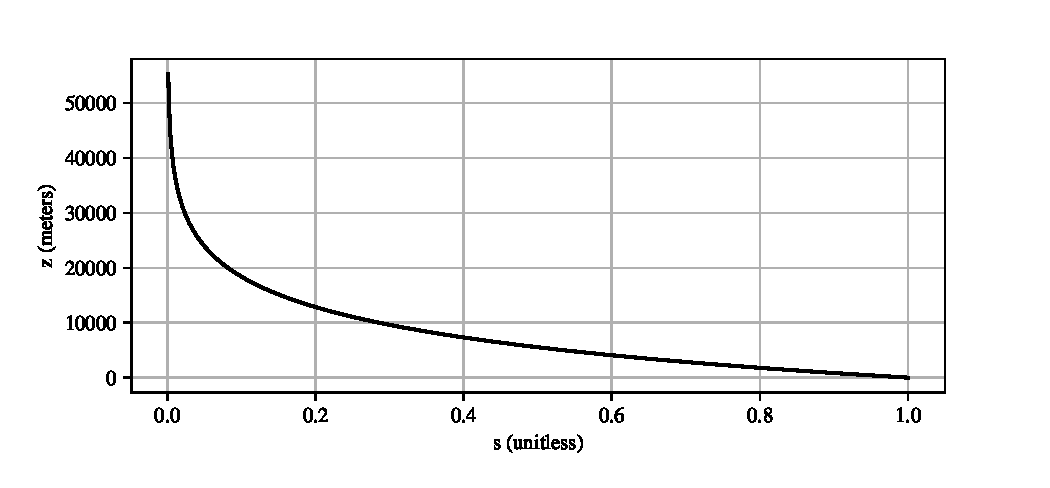
\includegraphics[width=.9\textwidth]{figures/s_to_z.pdf}}
    \caption{Transformation of $s$-coordinates to $z$-coordinates;
    both diagrams assume that $\pi (s)=s\cdot 1atm$, and $T=273K$, and use Eq.~\ref{eq_s_to_z} to translate an equidistant $s$-grid to a non-equidistant $z$-grid.
    The first diagram shows where each grid point is located in $z$-coordinates with $50$ grid points. 
    The second diagram shows the relationship between $s$-coordinates and $z$-coordinates.}
    \label{fig:s_grid}
\end{figure}
\begin{figure}[ht]
	\makebox[\textwidth]{ 
  		 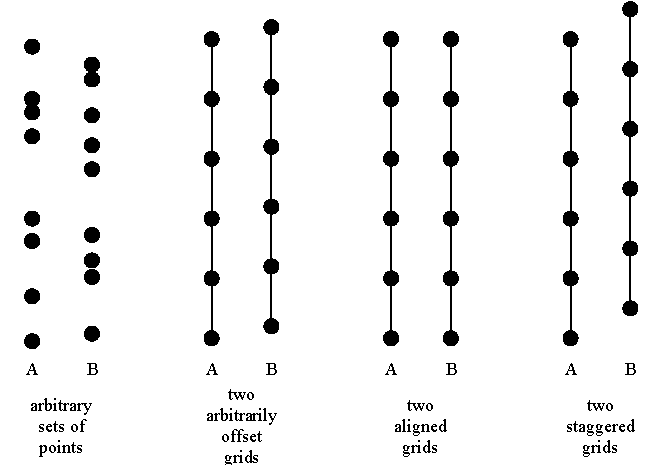
\includegraphics[width=.8\textwidth]{figures/discretization.pdf}}
    \caption{Different variants of discretization}
    \label{fig:grid_discretization}
\end{figure}
\begin{figure}[ht]
	\makebox[\textwidth]{ 
  		 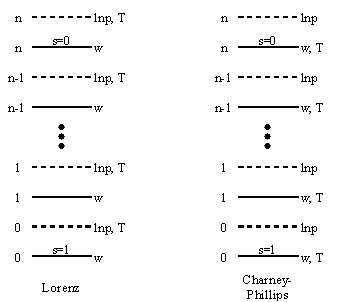
\includegraphics[width=.7\textwidth]{figures/lorenz_cp.pdf}}
    \caption{Variable distribution for Lorenz grid and Charney-Phillips grid}
    \label{fig:lorenz_cp}
\end{figure}
\noindent
When implementing the non-hydrostatic version of the NSE discussed in Section~\ref{sec:non_hydrostatic}, there are three prognostic variables to be considered: Vertical wind speed $w$, pressure $\text{ln}p$, and temperature $T$.
Each of them varies across the atmosphere and must thus be sampled at different points across space.
The question is where to place these points for each variable.

Generally speaking, every variable gets its own arbitrary set of points at which to sample.
In theory, the set of points could also vary over time.

To simplify calculation, we apply grids to bring order to the sets of points.
When a variable is sampled along a grid, it is sampled at every node of that grid.
In order to utilize the discrete differential operators from Section~\ref{section:diff_op}, the grids are chosen to be equidistant, i.e. the distance between two consecutive grid points (the mesh size) is always the same.
It is also assumed that the mesh size is the same for all three variables.

Note that in this context, the distance between grid points does not necessarily correspond to distance (measured in meters) in the real world.
This is due to the alternative coordinate system from Section~\ref{sec:non_hydrostatic} which transforms equidistant grid points in the s-coordinate-system to non-equidistant grid points in the z-coordinate system, depending on how the function $\pi(s)$ is defined.
This effect can be observed in Fig.~\ref{fig:s_grid}.


Having now established that all three variables ($\text{ln}p$, $T$, and $w$) are sampled along grids of equal mesh size, one remaining question is their relative placement.
In other words, the offset between two grids for two variables is a free parameter.
In case the offset is zero, we call the two grids aligned.
In case the offset is half the distance between two grid points, the two grids are called staggered.
To distinguish the two grids, we call one aligned, and the other offset.
This is illustrated in Fig.~\ref{fig:grid_discretization}.

For the NSE there are two prevailing staggered grid systems~\cite{holdaway2013comparison}: The Lorenz grid, and the Charney-Phillips grid which are shown in Fig.~\ref{fig:lorenz_cp}.
For the Lorenz grid, vertical wind $w$ is placed on the aligned grid, whereas pressure $\text{ln}p$ and temperature $T$ are on the offset grid.

For the Charney-Phillips grid, both vertical wind $w$ and temperature $T$ are placed on the aligned grid, and only pressure $\text{ln}p$ is on the offset grid.
The reason for always placing $w$ on the aligned grid, and pressure $\text{ln}p$ on the offset grid, is to enforce the boundary conditions discussed in Section~\ref{sec:boundary}.
By placing wind $w$ on the aligned grid, we can force $w_{top}$ and $w_{bottom}$ to be zero, since there are sample points both at the top and the bottom.

In contrast, with pressure $\text{ln}p$ it is advantageous not to have a sampling point at the upper boundary of the domain, as we may want to postulate pressure at the upper boundary to be zero, because the atmosphere is supposed to end there, i.e. $p_{top}=0$ which would mean $\text{ln}p = -\infty$.
To avoid dealing with non-computable numbers, pressure $\text{ln}p$ is placed on the offset grid.

We can place the remaining variable temperature $T$ on either the offset or the aligned grid, because it not affected by our boundary conditions.

\section{Discretization of Time and Types of Integrators}\label{sec:integrators}
Before we give examples of integrators, we must first define them.
An integrator is an algorithm that, given a starting condition $x(t_0) = x_0$, can solve a differential equation of the form $\frac{dx}{dt} = f(x,t)$, where $x$ is the state vector and $t$ is time.
Its goal is to generate a trace for $x(t)$ over time, after the starting time $t_0<t$.

\subsection*{Runge-Kutta Methods}
One of the simpler classes of integrators consists of the explicit Runge-Kutta methods.
These methods begin with the initial value $x_0$ and then create the trace $x(t)$ by making small time-steps $\Delta t$ starting at $t_0$ and modifying the state through addition: $x(t+h) = x(t) + RK(f,x,t,h)$.

The following derivation closely follows the derivation in~\cite{lyu2016plasma}.
Other derivations such as in~\cite{suli2003introduction} are also possible.
\\

\noindent
All Runge-Kutta methods aim to approximate the Taylor series expansion of $x(t)$ with respect to $t$, i.e.
\begin{align*}
x(t+h) &= x(t) + \sum_{k=1}^{n}\frac{h^k}{k!}\frac{d^kx}{dt^k} + \mathcal{O} \left(h^{n+1}\frac{d^{n+1}x}{dt^{n+1}}\right)\\
&= x(t)+ \sum_{k=0}^{n-1}\frac{h^{k+1}}{(k+1)!}\frac{d^kf(x(t),t)}{dt^k} + \mathcal{O}\left(h^{n+1}\frac{d^{n}f}{dt^{n}}\right)
\end{align*}
Exploiting $\frac{df(x(t),t)}{dt} 
= \frac{\partial f(x(t),t)}{\partial x}\frac{dx}{dt}+\frac{\partial f(x(t),t)}{\partial t} 
= f\frac{\partial f}{\partial x}+\frac{\partial f}{\partial t}$
this becomes.
\begin{align*}
x(t+h) &= x(t)+ \sum_{k=0}^{n-1}\frac{h^{k+1}}{(k+1)!}\left(\frac{\partial f}{\partial t} + f(x(t),t)\frac{\partial f}{\partial x}\right)^kf(x(t),t) + \mathcal{O}\left(h^{n+1}\frac{d^{n}f}{dt^{n}}\right)
\end{align*}
The simplest Runge Kutta method is the Explicit Euler or RK1 scheme which can be derived by writing down the Taylor expansion:
\begin{align*}
x(t+h) &= x(t) + h \cdot \frac{dx}{dt} + \mathcal{O}(h ^2)\\
&= x(t) + h \cdot f(x,t) + \mathcal{O}(h ^2)
\end{align*}
RK1 has a local truncation error of $\mathcal{O}(h^2)$, and a total accumulated error of $\mathcal{O}(h)$.
\\

\noindent
RK2 uses more than one evaluation of $f$ in order to do one step:
\begin{align*}
k_1 &= f(x(t),t)\\
k_2 &= f(x(t) + \frac{h}{2} k_1, t + \frac{h}{2})\\
&= f(x(t) + \frac{h}{2} f(x(t),t), t + \frac{h}{2})\\
&= f(x(t),t) + h\left(\frac{\partial f}{\partial t} + f(x(t),t)\frac{\partial f}{\partial x}\right)f(x(t),t) + \mathcal{O}(h^2)\\
&= f(x(t),t) + h\frac{df}{dt} + \mathcal{O}(h^2)\\
x(t) + \frac{h}{2} (k_1+k_2) &= x(t) + \frac{h}{2} \left(f(x(t),t) + f(x(t),t) + h\frac{df}{dt} + \mathcal{O}(h^2)\right)\\
&= x(t) + h f(x(t),t) + \frac{h^2}{2} \frac{df}{dt} + \mathcal{O}(h^3)\\
&= x(t) + h \frac{dx}{dt} + \frac{h^2}{2} \frac{d^2x}{dt^2} + \mathcal{O}(h^3)\\
\Rightarrow x(t+h) &= x(t) + \frac{h}{2} (k_1+k_2) + \mathcal{O}(h^3)
\end{align*}
RK2 has a local truncation error of $\mathcal{O}(h^3)$, and a total accumulated error of $\mathcal{O}(h^2)$.
\\

\noindent
In a similar fashion it can be shown that RK4 is:
\begin{align*}
k_1 &= f(x(t),t)\\
k_2 &= f\left(x(t)+\frac{h}{2}k_1,t+\frac{h}{2}\right)\\
k_3 &= f\left(x(t)+\frac{h}{2}k_2,t+\frac{h}{2}\right)\\
k_4 &= f(x(t) + h k_3, t + h)\\
x(t+h) &= x(t) + \frac{h}{6}(k_1+2k_2+2k_3+k_4)
\end{align*}
RK4 has a local truncation error of $\mathcal{O}(h^5)$, and a total accumulated error of $\mathcal{O}(h^4)$.

%\subsection{Exponential Integrators}
%In case $f(x,t)$ is a linear timeinvariant function, $f$ can be written as $f(x)=Ax$, where $A$ is a matrix.
%The resulting differential equation can be solved analytically, using the Laplace Transform which is explained in further detail in appendix \ref{sec:laplace_trafo}.
%To this end first, the Laplace transform is taken, and then the equation is solved for $X(s)$ (with $I$ being the identity matrix):
%\begin{align*}
%\frac{dx}{dt}(t) &= Ax(t)\\ 
%sX(s) - x(t_0) &= AX(s)\\
%X(s) &= (sI-A)^{-1}x(t_0)
%\end{align*}
%Thereafter the inverse Laplace transform can be taken to solve for $x(t)$:
%\begin{align*}
%x(t) &= \exp (A (t-t_0))x(t_0)\\
%\text{using:}~ \exp{At} &= I + \sum_{k=1}^{\infty}\frac{1}{k!}(At)^k
%\end{align*}
%As this is an analytic solution, it is exact and does not depend on step-size.
%However there are two major disadvantages to this method.
%First, if the system is not linear it needs to be linearized which makes the solution inexact.
%Second, it is comparatively slow as it requires a matrix to be exponentiated.
%Take, for example, the NSE discussed earlier.
%If temperature, wind speed, and density are stored at just 3000 grid points, this would entail the state vector $x$ having at least $3000\cdot 3=9000$ entries, and thus $A$ having $9000^2=8.1\cdot 10^7$ entries which would still be feasible to compute, just not fast, especially when compared to Runge-Kutta methods.\\
%As a countermeasure to the second issue, the matrix exponential can be approximated using several approaches.
%For further reading on this topic refer to~\cite{moler2003nineteen}.

%\begin{itemize}
%\item show how linear equations can be solved using laplace-%transforms and matrix exponentials
%\item give example of how matrix exponential can be approximated
%\end{itemize}


% !TeX root = ../main.tex
% Add the above to each chapter to make compiling the PDF easier in some editors.

\chapter{Implementation}\label{chapter:implementation}
In order to test the effects of the modifications and simplifications made in chapter \ref{chapter:navier_stokes}, and the effects of discretization described in chapter \ref{chapter:discretization}, everything discussed was implemented using a custom framework written in Python 3 with aid of the numpy-library.
The architecture of this framework will be described in this chapter.

\section{Design}
The framework was created keeping the design principle of modularity in mind.
This has several advantages.
First, it becomes possible to test and verify every component of the framework individually.
Second, it becomes easier to fulfill the goal of the framework, namely to test every possible configuration of simplifications and discretizations.
Modularizing these simplifications and discretizations makes it possible to switch between them easily.
\\
The functionality of the framework can be separated into two components. 
The first component is responsible for generating the data through either simulation or usage of analytic solutions.
This component is called Generator.
\\
The second component can then be used to evaluate the generated data, by using its error tracking and visualization\footnote{using matplotlib} capabilities.
This component is called Evaluator.

\subsection*{Generator}
Focusing on the data-generating component, its functionality was split up as follows:
\begin{itemize}
\item differential operators, modeled by functions. 
These functions take in a vector representing a scalar or vector field (represented by numpy-arrays), perform their respective operation on it, and return the result of the operation.
\item storing the system state in instances of the class \texttt{State}.
This class wraps a numpy-array storing the state variables, and the names of the all axes and variables.
\item differential equations, modeled by classes inheriting from the abstract class \texttt{TimeDerivative}.
When called and given an instance of \texttt{State}, objects of the \texttt{TimeDerivative} class calculate the time derivative given the current state, by applying the diagnostic equations of their respective differential equation to it.
\item integrators, modeled by classes inheriting from the abstract class \texttt{Integrator}.
During instantiation they receive an initial state and a differential equation (in the form of an \texttt{TimeDerivative} instance), which they are supposed to integrate, using a specified step size.
Every time an instance of \texttt{Integrator} is called it will integrate its differential equation by one step, advance its internal time by one step, and output the modified \texttt{State} instance.
\item analytic solutions to differential equations, modeled by classes inheriting from the abstract class \texttt{Solution}.
As these solutions are analytic, any time t can be specified, and an instance of \texttt{Solution} will output the state of the system modeled by its differential equation.
In order to be more similar to \texttt{Integrator} classes, they also contain an internal timer, which can be advanced by calling the instance of \texttt{Solution} without specifying a time t.
\end{itemize}
Using this separation into classes fulfills the objective of modularity.
For one, one \texttt{Integrator} class can be replaced for another without affecting other components of the program.
The same goes for different implementations of the same differential operators.
Second, for a given differential equation, it is possible to implement several different test scenarios or analytic solutions, by representing each by its own \texttt{Solution} class.
Last, it is possible to change the differential equation being simulated by changing the \texttt{TimeDerivative} class.
\\
As already mentioned above, as another design step taken for better readability, any class which repeatedly outputs new data was implemented as an iterator.
This includes all classes inheriting from \texttt{Integrator} and \texttt{Solution}, as they both generate new output for every iteration.
Using iterators makes code using repeated data-generation more compact and readable.

\subsection*{Evaluator}
The evaluator component builds on the premise that there is a solution (coming from a \texttt{Solution} object) and a calculated result (coming from an \texttt{Integrator} object).
Both calculated results and solutions are a discrete series of system states over time.
Within the program they are represented by a discrete series of \texttt{State} objects at monotonically increasing timestamps.
Of course there may be some differences between the solution and the calculated result, which will subsequently be called errors.
\\
The functionality of the component was split up as follows:
\begin{itemize}
\item the \texttt{ErrorTracker} class, which is used to store a series of errors, along with some kind of labeling (e.g. time, or spacial resolution).
Example: To store errors over time, every time step, an instance of \texttt{ErrorTracker} is given a timestamp as a label, the calculated result, and the solution at that timestamp.
From this it calculates the error (using a norm of the programmers choice) and stores it together with the timestamp.
\item the \texttt{ErrorIntegrator} class, which also calculates the error whenever it is given a calculated result and a solution, but then adds it its memorized total error, instead of storing it individually.
\item the \texttt{WindowManager} class is used for displaying both instances of \texttt{State} and of \texttt{ErrorTracker} visually.
Errors can be displayed both on a logarithmic and on an ordinary scale.
\\
For displaying \texttt{State} objects, the class also provides some functionality to apply a custom transformation to the data to be displayed, before displaying it.
\\
Example: When simulating, $\text{ln}p$ can be a diagnostic variable. In order to display $p$ instead of $\text{ln}p$, it needs to transformed through exponentiation first.
\end{itemize}

\subsection{Operators}
The smallest units of the framework are the operators.
Two categories of operators have been implemented: averaging operators, and the differential operators discussed in section \ref{section:diff_op}.\\
The averaging operators follow the naming scheme:
\\
\texttt{[operation abbreviation]\_e[error order]}
\\
where the error order indicates how many neighboring variables are taken into account when calculating the local average.
When considering a high spacial resolution, using more neighboring variables will make the estimation more accurate.\\
Example: Averaging samples of a function $f$ on an equidistant grid of mesh size $\Delta x$ by averaging each grid point with the following grid point.
\begin{figure}[htpb]
  \centering
  \begin{tabular}{c}
  \begin{lstlisting}[language=Python]
    f_average = avg_forward_e1(f, delta_x)
  \end{lstlisting}
  \end{tabular}
\end{figure}
\\
The differential operators follow the naming scheme:
\\
\texttt{[operation abbreviation]\_n[operator order]\_e[error order]}
\\ 
where the \texttt{operator order} can either be \texttt{1} for the first order derivative, or \texttt{2} for the second order derivative (also known as the laplacian).
The error order \texttt{e} is the exponent of $h$ in the error term $\mathcal{O}(h^\texttt{e})$ (see section \ref{section:diff_op}).\\
Example: calculating the derivative $\frac{df}{dx}$ of some function $f$ w.r.t. $x$ on an equidistant grid with mesh size $\Delta x$
\begin{figure}[htpb]
  \centering
  \begin{tabular}{c}
  \begin{lstlisting}[language=Python]
    df_dt = diff_n1_e2(f, delta_x)
  \end{lstlisting}
  \end{tabular}
\end{figure}

\subsection{Class Structure and Information Flow}
The interaction between the different types of classes is visualized in fig. \ref{UML_diagram}.

\begin{figure}[!h]
	\makebox[\textwidth]{ 
  		 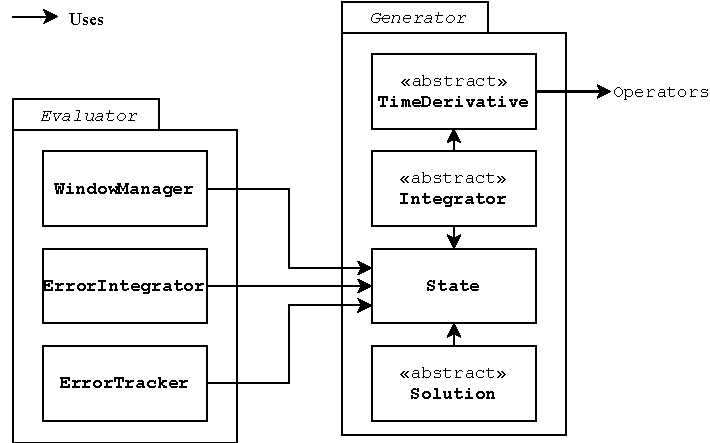
\includegraphics[width=.8\textwidth]{figures/UML.pdf}}
    \caption{UML-Style-Diagram}
    \label{UML_diagram}
\end{figure}

All communication between classes is done by passing references to \texttt{State}-objects.
As \texttt{State} objects can take up a lot of space in memory, passing them by reference is better than passing copies of them.
For the same reason, whenever possible, \texttt{State}-objects are reused to avoid overcrowding memory.
\\
During execution, both the \texttt{Integrator}- and the \texttt{Solution}-instance contain one \texttt{State}-object each.
Whenever new information is requested from them, they generate it, and return a reference to their internal \texttt{State}-object.
Now, the program that requested the information can use the \texttt{State}-objects.
To this end the Evaluator components can be used.

\subsection{Usage of the Framework}
Having established the framework with its abstract classes, in this section the way it is used is described, using the example of the wave equation with periodic boundary conditions\footnote{i.e. $u(x)=u(x+a)$ if $a$ is the periodicity} in the following form:
\begin{align*}
\frac{du}{dt} = \frac{dv}{dx}\\
\frac{dv}{dt} = c^2\frac{du}{dt}
\end{align*}
As was foreseen during design, there are multiple implementations of the abstract \texttt{Integrator}, namely implementations of RK1 (explicit Euler), RK2 (explicit Heun), RK4, and an implementation of an exponential integrator.
All of them can be found in the same folder.
\\
The remaining abstract classes are \texttt{TimeDerivative} and \texttt{Solution}.
Both of them are dependent on the differential equation to be simulated, and on the way it is simulated, i.e. different spacial discretizations/grids require new implementations of both \texttt{TimeDerivative} and \texttt{Solution}.
For this reason there is a separate folder for each differential equation to be analyzed.
Within each folder an appropriate implementation of \texttt{TimeDerivative} and \texttt{Solution} can be found.
\\
Using the example of the wave equation, the implementation of the \texttt{TimeDerivative}-class can be written as follows:\\
\begin{tabular}{c}
\begin{lstlisting}[language=Python]
class PeriodicWaveTimeDerivative(TimeDerivative):
  def __init__(self, delta_x, c):
    self.delta_x = delta_x
    self.c = c

  def __call__(self, state_vars, t):
    # extract the variables from the state variables
    u = state_vars[0]
    v = state_vars[1]
			
    # calculated the time-derivatives
    du_dt = diff_n1_e4(v, self.delta_x)
    dv_dt = self.c * self.c *  diff_n1_e4(u, self.delta_x)
        	
    # transform result into canonical format
    return np.stack((du_dt, dv_dt), axis=-1).transpose()
\end{lstlisting}
\end{tabular}\\
Using d'Alemberts solution, which dictates that for a starting condition of $u(x,t=0)=f(x)$ and $v(x,t=0)=0$, the solution can be written as $u(x,t)=\frac{1}{2}(f(x+ct)+f(x-ct))$ and $v(x,t)=\frac{c}{2}(f(x+ct)-f(x-ct))$, one possible implementation of the \texttt{Solution}-class can be written as follows:\\
\begin{tabular}{c}
\begin{lstlisting}[language=Python]
class WaveEqSolution(Solution):
  def __init__(self, num_grid_points, dt, domain_size, c, f):
    super().__init__(0, dt)
    # store all variables necessary for calculating the solution
    self.c = c
    self.f = f
    # create the grid along which to sample u and v
    self.x = np.tile(np.linspace(0, domain_size, num_grid_points + 1)[:-1],
                       (2, 1))
    # create an instance of State-class
    self.state = utils.State(num_vars=2, dim_vars=num_grid_points,
                         axes=self.x, names=[("x", "u"), ("x", "v")])

  def solution(self, t): # according to D'Alembert
    # u = state_vars[0] and v = state_vars[1]
    state_vars = self.state 
        
    # calculate the result
    state_vars[0] = 0.5 * (self.f(self.x[0] + t * self.c)
                             + self.f(self.x[0] - t * self.c))
    state_vars[1] = self.c * 0.5 * (self.f(self.x[0] + t * self.c)
                                       - self.f(self.x[0] - t * self.c))

    return self.state
\end{lstlisting}
\end{tabular}
\\
To now put everything together, the modus operandi is as follows:
First, an initial state of the system must be defined.
If the calculated result should be compared against an analytic solution, the initial state can be gained by first creating an instance of \texttt{Solution}, and then asking it for the system state at time $0$.
Otherwise one can directly create an instance of \texttt{State} and set its initial conditions manually.
\\
In the example there is a solution so the starting condition can be gained as follows:\\
\begin{tabular}{c}
\begin{lstlisting}[language=Python]
# creating an instance of WaveEqSolution
solver = WaveEqSolution(num_grid_points, dt, domain_size, c, f)
initial_state = solver.solution(t=0)
\end{lstlisting}
\end{tabular}
\\
Next, an instance of \texttt{TimeDerivative} must is created.\\
\begin{tabular}{c}
\begin{lstlisting}[language=Python]
# calculate mesh size
delta_x = domain_size / num_grid_points
# creating an instance of PeriodicWaveTimeDerivative
time_derivative = PeriodicWaveTimeDerivative(delta_x, c)
\end{lstlisting}
\end{tabular}\\
Both this instance and the instance of \texttt{State} containing the starting conditions of the system are necessary to create an instance of \texttt{Integrator}.\\
\begin{tabular}{c}
\begin{lstlisting}[language=Python]
# creating an instance of RungeKutta.Explicit
integrator = RungeKutta.Explicit(initial_state, time_derivative, t0=0,delta_t=dt)
\end{lstlisting}
\end{tabular}
\\
Now, depending on what the aim of the simulation is, the appropriate instances from the Evaluator components can be instantiated, which concludes the setup.
\\
As both \texttt{Integrator} and \texttt{Solution} are implemented as iterators, the system can simulated by using a simple \texttt{for}-loop.
As an iterator, \texttt{Integrator} will return the calculated result, and \texttt{Solution} will return the analytic result.
This means that within the \texttt{for}-loop the programmer has access to the accurate result, the analytic result, and can now perform any further necessary operations on those results.\\
\begin{tabular}{c}
\begin{lstlisting}[language=Python]
for int_state, sol_state in zip(integrator, solver): 
  # do operations on the states
\end{lstlisting}
\end{tabular}
\\
For some of the most common operations a programmer might want to do within the \texttt{for}-loop, a function performing the entire setup has been preimplemented in the \texttt{run\_ utils.py} file.
\\
Another helpful preimplementation is that of the numerical reference solution.
It can be used whenever no analytic solution is known, but a reference solution is still required.
In this case, a reference solution is created by simulating the differential equation using RK4 and doing very small time-steps.
To avoid having to re-calculate this, the result of this time-intensive simulation is stored to the disk.

\section{Testing}\label{sec:testing}
While it is not possible to mathematically prove that the implementation is without fault, the next best thing is exhaustive testing.
For this framework testing usually entails checking the outputs of the components against a reference solution, which was found separately.
This reference solution is usually analytic in nature and has to be derived through manual calculation.
\\
The approach taken to test the framework was bottom-up, i.e. first, the smallest possible components were tested in isolation, then, components using only tested sub-components could be tested, too.
In the following the tests for the Generator components are described.

\subsection{Operators}
In the case of this framework the smallest component are the operators.
They were tested using operations simple enough that a simple analytic expression exists.
Then the result of the numerical operator was compared against this analytic expression.
For the averaging operators this step was sufficient.
\\
In order to further verify the derivative operators, the order of the error was also checked, i.e. after changing the spacial resolution by a factor of $a$, an operator of the $n$-th error order was expected to reduce its error by a factor of $a^n$.

\subsection{Integrators}
In order to test the integrators separately from the differential operators, single-variable differential equations were used.
Having only one variable and no spacial dimension means spacial derivative operators do not have to be utilized.
For testing purposes four such differential equations for which analytic solutions exist, were implemented as subclasses of  \texttt{TimeDerivative} and \texttt{Solution}.
Having isolated the Integrator as the component to be tested (as much as possible), it is then run at different resolutions.
For Runge Kutta methods of order $n$ an increase in resolution by a factor of $a$ was expected to reduce error by a factor of $a^n$.
However, for exponential integrators this method fails, as exponential integrators are either accurate down to machine precision or wholly inaccurate.
For them, instead, a very small error was sufficient in order to complete the test.

\subsection{Differential Equations}
Having verified the implementation of both operators and integrators, the only component left to verify are the implementations of the differential equations in the form of \texttt{TimeDerivative}-implementations.
The process for this is similar to the previous sections: First, some analytic solution is found.
The breadth of this analytic solution can vary in its universality.
From analytic solutions describing the evolution of the system given any starting condition\footnote{which makes a numeric solutions redundant}, to analytic solutions describing the stationary solution of the system.
A stationary solution is a solution for which the state of the system does not change.
This solution is then implemented as a \texttt{Solution} class.
\\
After finding such an analytic solution, its initial state is given to an integrator (usually RK4), which uses the \texttt{TimeDerivative}-implementation to be tested in order to calculate its results independently from the analytic solution found.
\\
Now running both the analytic solution and the calculated simulation, these two results can be compared.
If the results are coinciding, chances are good the implementation of \texttt{TimeDerivative} was correct.
To further verify the solution, one can also vary the resolution with which RK4 is run.
If change in resolution by a factor of $a$ translates into a reduction in error by a factor of $a^4$, this is a good indicator that the solution described by \texttt{TimeDerivative} converges towards the analytic solution, which was found separately.

\subsection{Example}
Now that the implementation architecture has been detailed, the implementation of the non-hydrostatic NSE in the form of a \texttt{TimeDerivative}-implementation is explained.
More specifically an implementation of the Lorenz-grid is shown.\\
First off, the variables used in the implementation are detailed:\\
{\tabulinesep=0.5mm
\begin{center}
\begin{tabu}{c|c|c}
\hline 
Variable Name & Type & Meaning \\ 
\hline 
\texttt{delta\_s} & scalar & mesh size/distance between $s$-grid points \\ 
\hline 
\texttt{s} & vector & \makecell{vector containing the $s$-locations\\of all grid nodes of the aligned grid.}\\ 
\hline 
\texttt{dpi\_ds}& function & this represents $\frac{\partial\pi}{\partial s}$ \\ 
\hline 
\texttt{state\_vars} & 2d-array/list of vectors & \makecell{contains the state-variables.\\$\text{ln}p$=\texttt{state\_vars[0]}\\ $T$=\texttt{state\_vars[1]}\\ $w$=\texttt{state\_vars[2]}}\\ 
\hline 
\texttt{t} & scalar & \makecell{contains the elapsed simulation time\\(is not used in this implementation).} \\ 
\hline 
\texttt{lnp} & vector & contains all samples of $\text{ln}p$ \\
\hline 
\texttt{p} & vector & contains all samples of $p$ \\
\hline 
\texttt{T} & vector & contains all samples of $T$ \\ 
\hline 
\texttt{w} & vector & contains all samples of $w$ \\ 
\hline 
\texttt{dlnp\_dt} & vector & contains all samples of $\frac{\partial\text{ln}p}{\partial t}$ \\
\hline 
\texttt{dT\_dt} & vector & contains all samples of $\frac{\partial T}{\partial t}$ \\ 
\hline 
\texttt{dw\_dt} & vector & contains all samples of $\frac{\partial w}{\partial t}$ \\ 
\hline 
\end{tabu} 
\end{center}}

The only two operators utilized are the following:\\
\begin{tabular}{c}
\begin{lstlisting}[language=Python]
diff_s_align_n1_e2(f_offset, delta_s)
diff_s_offset_n1_e2(f_aligned, delta_s)
\end{lstlisting}
\end{tabular}\\
Both functions approximate the derivative using central differences with a twist.
Usually, when central differences are calculated, if the input is on an aligned grid, the output will also be on an aligned grid.
This means the derivative at location $f(s)$ is approximated using values at $f(s-\Delta s)$ and at $f(s+\Delta s)$.
In contrast, \texttt{diff\_s\_offset\_n1\_e2} takes its input on an aligned grid, and outputs it on an offset grid.
That is, the derivative at location $f(s)$ is approximated using the values at $f(s-\frac{\Delta s}{2})$ and $f(s+\frac{\Delta s}{2})$.
Vice versa, \texttt{diff\_s\_offset\_n1\_e2} takes its input on an offset grid, and outputs it on an aligned grid.\\
Using these definitions, implementation of the non-hydrostatic NSE is reasonably simple.
When reading the code, note the close relation to the mathematical notation, which can be seen best by writing them down side by side:
\paragraph{Evolution of Vertical Wind Speed:}
\begin{align*}
\frac{\partial w}{\partial t} = -g\left(1 - \frac{\partial p}{\partial s}\left(\frac{\partial \pi}{\partial s}\right)^{-1}\right)
\end{align*}
\begin{center}
\begin{tabular}{c}
\begin{lstlisting}[language=Python]
dw_dt =
- const.g * (1 - diff_s_align_n1_e2(p, self.delta_s) / self.dpi_ds(self.s))
\end{lstlisting}
\end{tabular}
\end{center}

\paragraph{Evolution of Pressure}
\begin{align*}
\frac{\partial \text{ln}p}{\partial t} = \frac{g}{1- \frac{R}{C_p}} \frac{p}{RT}\left(\frac{\partial \pi}{\partial s}\right)^{-1} \frac{\partial w}{\partial s}
\end{align*}

\begin{center}
\begin{tabular}{c}
\begin{lstlisting}[language=Python]
dlnp_dt = (const.g / (1 - const.R / const.C_p)) 
           * (p / (const.R * T)) 
           * diff_s_offset_n1_e2(w, self.delta_s) 
           / self.dpi_ds(self.s + self.delta_s / 2)
\end{lstlisting}
\end{tabular}
\end{center}

\paragraph{Evolution of Temperature}
\begin{align*}
\frac{\partial T}{\partial t} = \frac{RT}{C_p}\frac{\partial \text{ln}p}{\partial t}
\end{align*}

\begin{center}
\begin{tabular}{c}
\begin{lstlisting}[language=Python]
dT_dt = (const.R / const.C_p) * T * dlnp_dt
\end{lstlisting}
\end{tabular}
\end{center}

\begin{tabular}{c}
\begin{lstlisting}[language=Python]
class LorenzTimeDerivative(TimeDerivative):
  def __init__(self, delta_s, s, dpi_ds):
    # store the variables necessary for computation
    self.delta_s = delta_s
    self.dpi_ds = dpi_ds
    self.s = s

  def __call__(self, state_vars, t):
    # extract the state variables from the system state
    lnp = state_vars[0]
    p = np.exp(lnp)
    T = state_vars[1]
    w = state_vars[2]
	
    # prognostic equation for pressure (offset grid)
    dlnp_dt = (const.g / (1 - const.R / const.C_p)) \
               * (p / (const.R * T)) \
               * diff_s_offset_n1_e2(w, self.delta_s) \
               / self.dpi_ds(self.s + self.delta_s / 2)
    
    # prognostic equation for temperature (offset grid)
    dT_dt = (const.R / const.C_p) * T * dlnp_dt
    
    # prognostic equation for vertical wind (aligned grid)
    dw_dt = - const.g \ 
    * (1 - diff_s_align_n1_e2(p, self.delta_s) / self.dpi_ds(self.s))
	
    # boundary conditions
      # index 0 <=> s=0 <=> top of atmosphere
      # index -1 <=> s=1 <=> bottom of atmosphere
    # fix pressure to 0 (ln(0)=-inf) above atmosphere
    dlnp_dt[0] = 0  
    # fix temperature outside atmosphere to be same as at top of atmosphere
    dT_dt[0] = dT_dt[1]
    # set wind at top and bottom to stay constant at zero
    dw_dt[0] = 0 
    dw_dt[-1] = 0

    # transform result into canonical format
    return np.stack((dlnp_dt, dT_dt, dw_dt), axis=-1).transpose()
\end{lstlisting}
\end{tabular}\\


%\begin{itemize}
%\item Lorenz-Grid
%\item introduce used variables
%\item show equivalence between symbolic math and code
%\item show how to enforce boundary conditions
%\end{itemize}
\chapter{Numerical Studies}
Having discussed how the NSE were simplified, discretized, and implemented, in this section the implementation is tested and validated.
To this end, first the results of the unit tests from section \ref{sec:testing} are discussed by looking at the numerical errors made by the differential operators and integrators.
Thereafter the implementations of the non-hydrostatic NSE discussed in section \ref{sec:non_hydrostatic} are analyzed.

\section{Validation by Analyzing Numerical Errors}
In this section the results of the tests performed in section \ref{sec:testing} are discussed.

% analysis of errors
\subsection{Differential Operators}
To test the differential operators, the function $f(x)=\sin(20\pi (x-e))$ was used on the domain $[0;1]$.
The offset of $e$ was introduced in order to avoid random perfect results.
Without it, if, for example, the samples happen to be located at the maximums, minimums and zero-crossings, even a simple central difference would make zero error.
With an offset of an irrational number, such as $e$, this is improbable.\\
For this test function the analytic result is the derivative $\frac{df}{dx}=20\pi\cos(20\pi (x-e))$.\\
To test the different methods of calculating the derivative numerically, the domain was sampled at resolutions ranging from $5$ to $20\cdot 10^7$ samples, which were spread equidistantly over the domain.\\
First, looking at the implementation of the finite differences.
If their implementation is correct, one would expect the error \texttt{finite\_ difference} $(x)-\frac{df}{dx}$ to drop with growing resolution.
More specifically for a finite difference operator of order $n$, when increasing the number of samples by a factor of $a$ one would expect a decrease in error of magnitude $a^{-n}$.
The positive result of the test can be seen in Fig. \ref{fig:derivative_error}.
\begin{figure}[!h]
	\makebox[\textwidth]{ 
  		 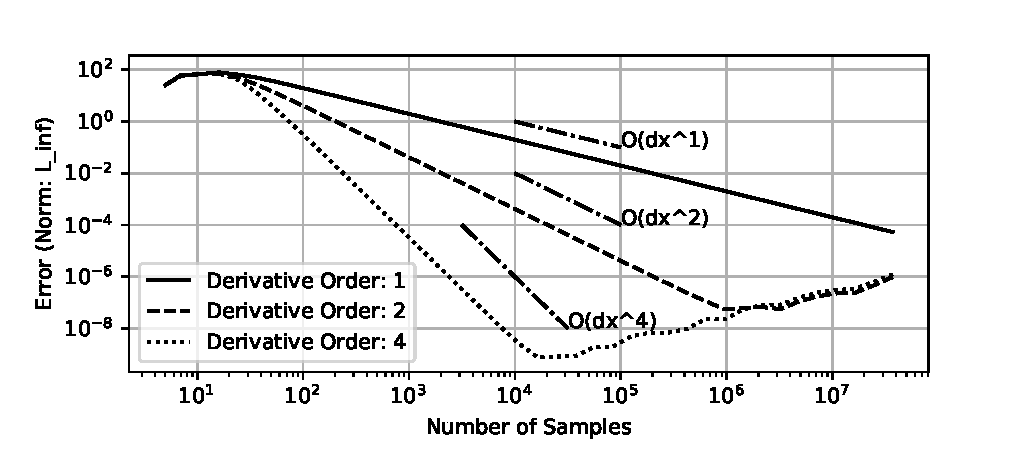
\includegraphics[width=1.2\textwidth]{figures/derivative_error.pdf}}
    \caption{Plot of error of finite difference operators over number of samples}
    \label{fig:derivative_error}
    \small
    The lines are parallel to the expected error order lines, meaning the test was successful.
\end{figure}
It can also be seen that above a certain spacial resolution, the error increases again, which is due to numerical errors.
The root of these errors is the division of a very small number in the denominator by the small number $\Delta x$, which is inversely proportional to the resolution.
This division of small numbers is not well-supported by floating point numbers, and for that reason errors will increase above a certain spacial resolution.\\
Looking at the implementation of the spectral derivative, it is expected that the error will drop down to machine precision as soon as the Nyquist sampling rate is reached.
The Nyquist sampling rate is twice the highest frequency occurring in the signal whose derivative is to be calculated.
In this case the highest frequency is $10$, because the argument of $\sin$ was $2\pi\cdot 10$, meaning the Nyquist sampling rate is $20$.
The fact this theoretical result can be observed in practice (Fig. \ref{fig:fft_error}), is a strong indication that the implementation is correct.

\begin{figure}[!h]
	\makebox[\textwidth]{ 
  		 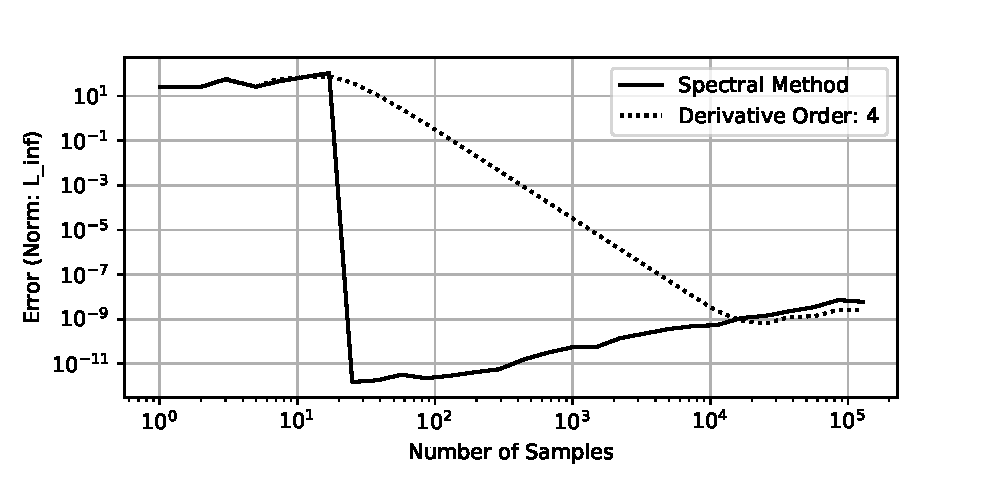
\includegraphics[width=1.2\textwidth]{figures/fft_error.pdf}}
    \caption{Plot of error of spectral derivative operator over number of samples}
    \label{fig:fft_error}
    \small
    As expected the error drops significantly as soon as the Nyquist sampling rate (20 samples) is reached.
\end{figure}

%Test-Function: $\sin(20\pi (x-e))$ on domain $[0;1]$, with resolutions from 5 to $20\cdot 10^7 $
%Actual result is $20\pi\cos(20\pi (x-e))$\\
%show how the error-order is influenced by grid-size.\\
%grid size far larger than features to be measured => inaccuracy\\
%grid size a little bit smaller than features to be measured => change in accuracy according to error-order of implemented operator\\
%grid size too small for machine precision => loss of accuracy

\subsection{Integrators}
\subsubsection{Runge-Kutta-Integrators}
As described in section \ref{sec:testing} the integrators were tested by comparing the results to analytic solution of differential equations.
Specifically, they were first tested against three types of differential equations, whose solutions are known analytically.
The first one was time-invariant and had only one variable, i.e. no spacial resolution.
The second one introduced time-variance into the mix, while the third one added spacial resolution.
In each of the tests, using a Runge-Kutta integrator of order $n$ it was expected that decreasing the time step size by a factor of $a$ would decrease the error by a factor of $a^n$.\\
\paragraph*{Time-Invariant, Single Variable}
The differential equation used is $\frac{dx}{dt}=-3x$, which has the solution $x(t)=x_0e^{-3t}$.
The result of the experiment can be seen in Fig. \ref{fig:RK_error_y'=-3y}.
\begin{figure}[!h]
	\makebox[\textwidth]{ 
  		 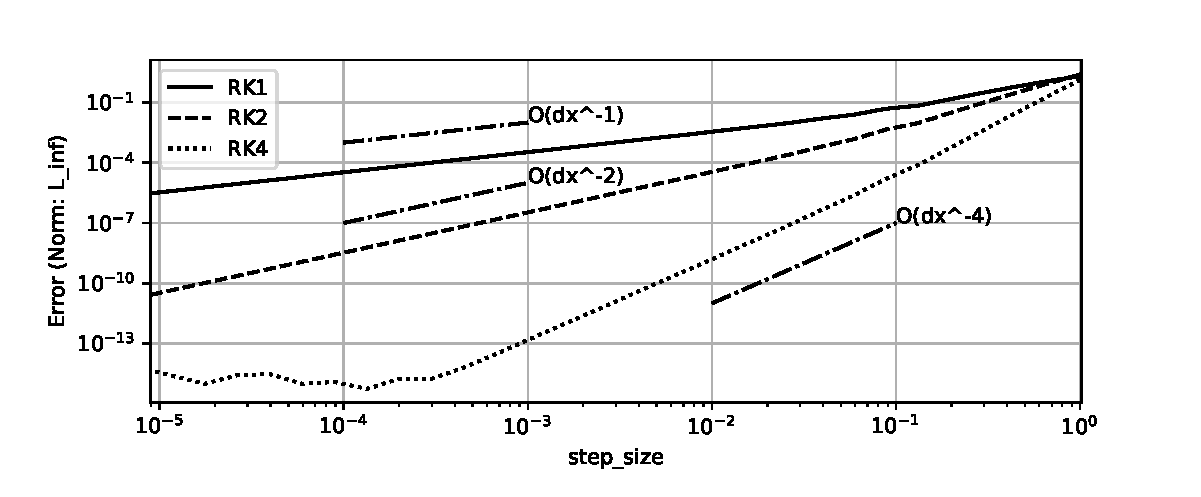
\includegraphics[width=1.2\textwidth]{figures/RK_error_y'=-3y.pdf}}
    \caption{Error of RK-methods on time-invariant, single variable differential equation}
    \label{fig:RK_error_y'=-3y}
\end{figure}

\paragraph*{Time-Variant, Single Variable}
The differential equation used is $\frac{dx}{dt}=\frac{t}{t^2+1}$, which has the solution $x_0 + 0.5\text{ln}(t^2+1)$.
The result of the experiment can be seen in Fig. \ref{fig:RK_error_y'=tdiv(t_t+1)}.
\begin{figure}[!h]
	\makebox[\textwidth]{ 
  		 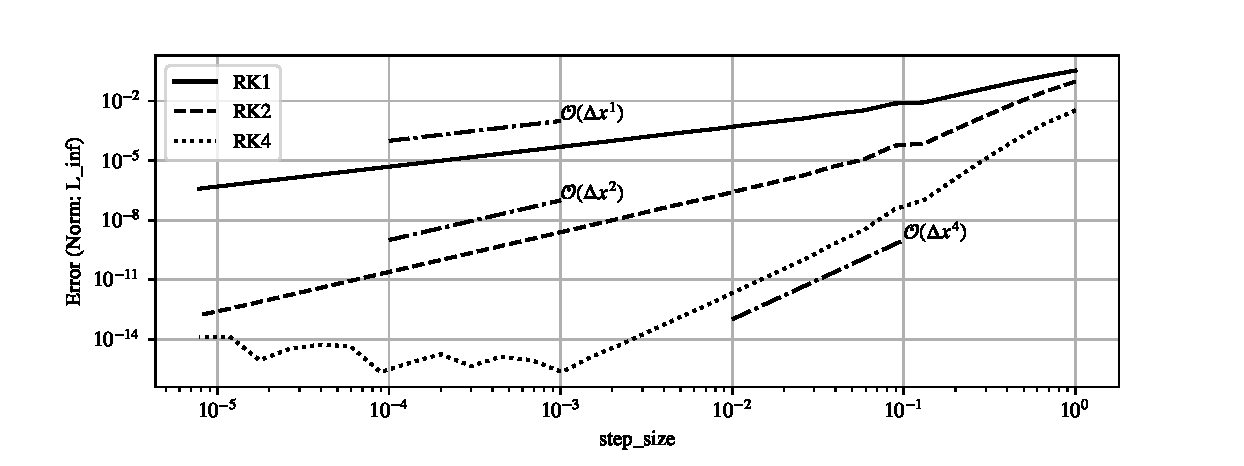
\includegraphics[width=1.2\textwidth]{figures/RK_error_y'=tdiv(t_t+1).pdf}}
    \caption{Error of RK-methods on time-variant, single variable differential equation}
    \label{fig:RK_error_y'=tdiv(t_t+1)}
\end{figure}

\paragraph*{Time-Invariant, Multiple Spatially Distributed Variables}
The differential equation used is the wave equation with periodic boundary conditions.
With $c$ being the wave propagation speed, the equation system can be written as follows:
\begin{align*}
\frac{du}{dt}&=\frac{dv}{dx}\\
\frac{dv}{dt}&=c^2\frac{du}{dx}
\end{align*}
If $u(x,t=0)=f(x)$ (with $f$ being periodic) describes the initial state of $u$, then according to d'Alembert the solution is $u(x,t)=\frac{1}{2}(f(x+ct)+f(x-ct))$, which means $v(x)=\int \frac{du}{dt} dx = \frac{c}{2}(f(x+ct)-f(x-ct))$.

\begin{figure}[!h]
	\makebox[\textwidth]{ 
  		 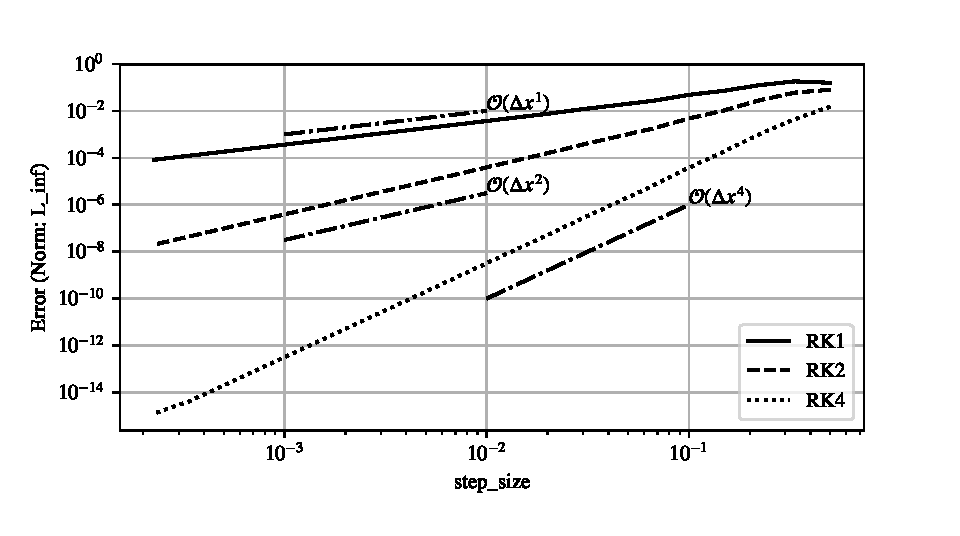
\includegraphics[width=1.2\textwidth]{figures/wave_order_line.pdf}}
    \caption{Error of RK-methods on periodic wave equation}
    \label{fig:wave_order_line}
\end{figure}

Interestingly, spacial resolution and temporal resolution are intertwined, i.e. if a very high spacial resolution (a lot of samples) is chosen, one also has to choose a high temporal resolution (small time steps).
This can be seen when plotting a heatmap of the error made when using the RK4-integrator over different spacial and temporal resolutions.
This phenomenon can be seen in Fig. \ref{fig:heatmap_wave_eq_step_size_numgridpoints}.
Roughly speaking, in order to keep the error from blowing up, an inverse proportion between spacial resolution and time step size should be kept, i.e. when doubling the spacial resolution, one should at least halve the time step size, in order to stay stable.

\begin{figure}[!h]
	\makebox[\textwidth]{ 
  		 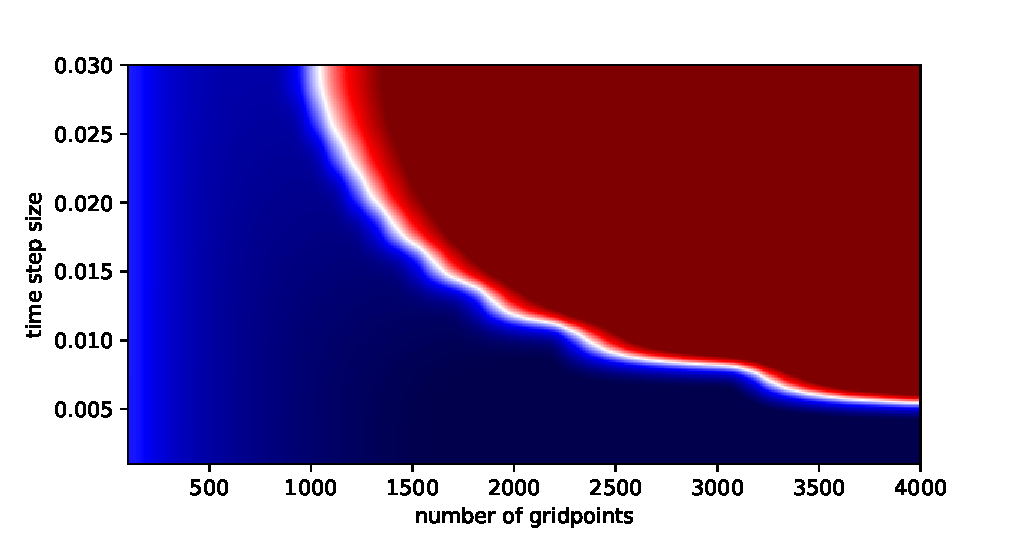
\includegraphics[width=1.2\textwidth]{figures/heatmap_wave_eq_step_size_numgridpoints.pdf}}
    \caption{Heatmap of log(Error) for wave equation over different spacial and temporal resolutions}
    \label{fig:heatmap_wave_eq_step_size_numgridpoints}
	\small
The white stripe represents the area where the log-error is 0, i.e. the actual error is 1.
The red area represents the area where the log-error is positive (can reach values up to $150$), i.e. large.
The blue area represents the area where the log-error is negative (can reach values down to $-20$), i.e. small.
\end{figure}

%$frac{dx}{dt}=\frac{t}{t^2+1}$, which has the solution $x_0 + 0.5\text{ln}(t^2+1)$.



%a time-invariant differential equation with only one variable (i.e. no spacial resolution), then a time-variant differential equation with no spacial resolution, and finally against a differential.
%First off, to verify the implementation, the RK-Integrators were used to solve a differential equation without any spacial resolution, but with temporal variance.
%$\frac{dx}{dt}=\frac{t}{t^2+1}$
%with solution $x_0 + 0.5\text{ln}(t^2+1)$.

%explain how time-step-size and grid-size have to change together, and show trough examples how accuracy changes depending on the choice of these two parameters (maybe a heatmap with x-axis = time-step-size, y-axis=grid-size, color=accuracy after simulation time T?)
%\subsubsection{Exponential Integrators}
%showcase how accuracy stays constant independent of time-step-size (for linear systems)\\
%give a small example of simulating a non-linear system by linearization around the current state


\section{Study of Errors in Implementation of NSE}
In this section the two implementations of the NSE are analyzed.
As no benchmarking systems for testing the vertical of the non-hydrostatic NSE-equations in isolation exist, true verification of the implementation is not possible.
Instead, four tests will be considered:
\begin{itemize}
\item comparison with a stationary solution
\item comparison of stationary solution with real world measurements
\item energy conservation
\item comparison of the two implementations to one another
\end{itemize}

\subsection{Comparison with Stationary Solution}
To find a stationary solution for the non-hydrostatic NSE, all time-derivatives have to be set to zero:
\begin{align}
\frac{\partial w}{\partial t} =0&= -g\left(1 - \frac{\partial p}{\partial s}\left(\frac{\partial \pi}{\partial s}\right)^{-1}\right)\label{stat_dw_dt} \\
\frac{\partial \text{ln}p}{\partial t}=0 &= \frac{g}{1- \frac{R}{C_p}} \frac{p}{RT}\left(\frac{\partial \pi}{\partial s}\right)^{-1} \frac{\partial w}{\partial s}\label{stat_dlnp_dt}\\
\frac{\partial T}{\partial t} =0&= \frac{RT}{C_p}\frac{\partial \text{ln}p}{\partial t}\label{stat_dT_dt}
\end{align}
The first equation \ref{stat_dw_dt} yields the following identity for pressure:
\begin{align*}
\frac{\partial p}{\partial s}=\left(\frac{\partial \pi}{\partial s}\right)\\
\Rightarrow p(s)=\pi (s) + p_0
\end{align*}
The second equation \ref{stat_dlnp_dt} is requires one of the elements in the denominator to equal zero.
As neither $g$, $p$, nor $\left(\frac{\partial \pi}{\partial s}\right)^{-1}$ can be zero, the only possible option is that $\frac{\partial w}{\partial s}=0$, i.e. $w(s)=w_0 \forall s$.
Due to the boundary conditions, at the bottom of the atmosphere $w(1)=0$, so $w(s)=w_0 \forall s$.\\
The last equation \ref{stat_dT_dt} yields no information, because the right hand side is already zero, due to $\frac{\partial \text{ln}p}{\partial t}=0$.
This means $T$ can be chosen freely, e.g. $T=273K$.\\
Using this stationary solution to define the initial state of the system, the integrator is expected not to change the system state.
This is reflected by both implementations as can be seen in Fig. 

\begin{figure}[!h]
	\makebox[\textwidth]{ 
  		 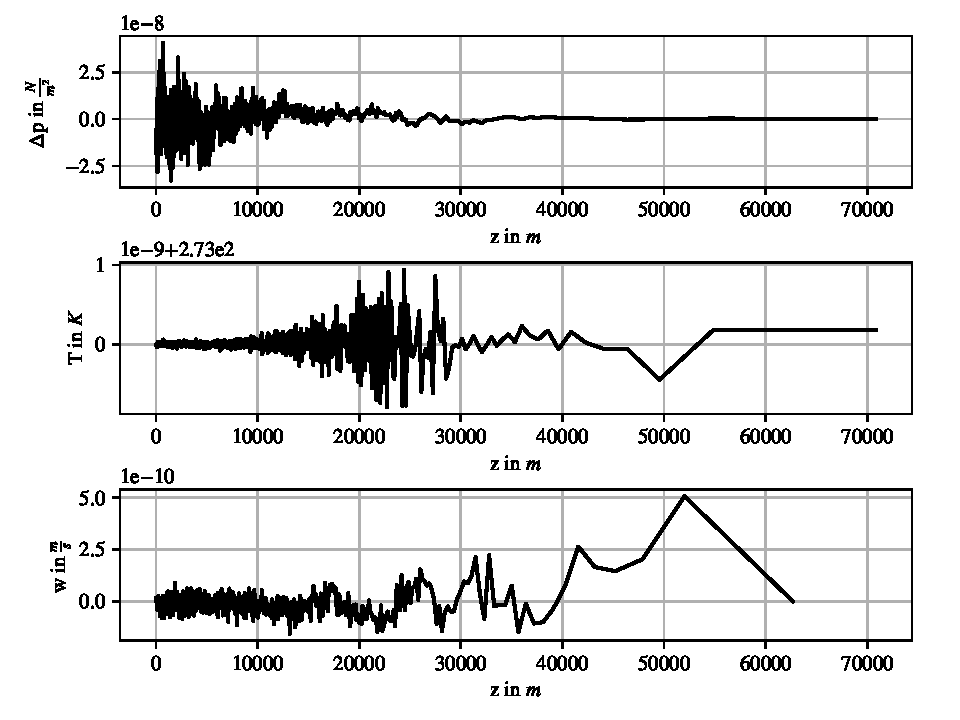
\includegraphics[width=1.2\textwidth]{figures/lorenz_240s_stat.pdf}}
    \caption{Error (deviation from stationary solution) made using RK4, time-step-size $2.5ms$, and $1000$ grid points, after $240s$ of simulation time}
    \label{fig:lorenz_stat_err}
\end{figure}

%In this section the effects (all?) possible choices of simplifications, integrators etc. is analyzed.\\
%To this end we introduce different ways of measuring errors, i.e. different norms, and use them to measure the difference between different simulations.

%\subsection{Simplifications to the Navier Stokes Equations} % effects of simplifications
%have one simulation without simplifications run with high precision (RK4 with tiny step-sizes and high grid resolution), and compare that to simulations using high precision with simplifications.

\subsection{Grid Discretizations}% grid discretizations
Quantify the difference between the two different grids.
How do we really know which one is better?
Find ways to quantify which one is more accurate?
% !TeX root = ../main.tex
% Add the above to each chapter to make compiling the PDF easier in some editors.

\chapter{Conclusion}\label{chapter:conclusion}
In this chapter we summarize the thesis and suggest some possible areas of future work based on the Python tool.
The code is freely available for this purpose as a Github repository at \url{https://github.com/Linus-H/Vertical-Integration}.

\section{Summary}
In this thesis we first gave a basic introduction to the Navier Stokes Equations for numerical weather prediction.
Having defined the most general equation system, we then rearranged and simplified this system, by assuming that horizontal wind $\textbf{V}$ is zero.
Thereafter, we substituted the variable $z$ by a new vertical coordinate $s$ which leads to a new equation system with some advantageous properties.
For example, the substitution leads to a high spatial resolution in the lower areas of the atmosphere in contrast to the low spatial resolution at the top of the atmosphere.
On top of this, this substitution allows for the upper bound for the domain to be found dynamically instead of setting it at the beginning of the simulation manually.
We employed the resulting equation system in the later sections.

Having established the version of the NSE to be simulated in Chapter~\ref{chapter:navier_stokes}, we explained the applied methodology for spatial and temporal discretization in Chapter~\ref{chapter:discretization}.
Then we outlined the modular framework of the software in Chapter~\ref{chapter:implementation}, and we gave an example of an implementation at the end of the chapter.
Finally, we described the tests conducted on the implementation and their results in Chapter~\ref{chapter:numerical_study}.


\section{Future Work}
There are multiple directions in which the the work done in this thesis can be expanded.
The first category consists of more experiments that could be conducted on the non-hydrostatic equation system.
\begin{itemize}
\item Observing the effects of varying temporal and spatial resolution; the effects would be expected to be quite significant, as the non-hydrostatic equation system is non-linear.
\item Experimenting with other time integrations methods/other integrators, to see whether they yield significantly different results from the Runge-Kutta-methods primarily used in this thesis.
\item Measuring the wave-speeds/speed of sound of waves at different wave-lengths. 
\end{itemize}
The second category of possible expansion are comparative in nature:
\begin{itemize}
\item compare the simulation results of the non-hydrostatic NSE to simulation results from implementations with the hydrostatic NSE.
\item compare the non-hydrostatic implementation to real-world measurements, by adding the remaining two dimensions of the horizontal to the implementation.
\end{itemize}
Lastly, it would be interesting to define standardized benchmarks for the non-hydrostatic NSE.
So far, such benchmarks are mainly adopted for systems employing the hydrostatic NSE~\cite{williamson1992standard}, making standardized comparisons between different implementations of then non-hydrostatic NSE difficult.


\appendix{}
\chapter{Appendix}
\begin{align*}
\mathcal{L}\{x(t)\}=X(s)=\int_0^\infty x(t)\exp (-st)dt
\end{align*}
For differential equations the identity for derivatives is key:
\begin{align*}
\mathcal{L} \left\{ \frac{dx}{dt}(t) \right\} &=\int_0^\infty \frac{dx}{dt}(t)\exp (-st)dt\\
&=x(t)\exp(-st)\rvert _0^\infty + s  \int_0^\infty x(t)\exp (-st)dt\\
&=-x(t=0) + sX(s)
\end{align*}


\microtypesetup{protrusion=false}
%\listoffigures{}
%\listoftables{}
\microtypesetup{protrusion=true}
%\bibliographystyle{abbrv}
\bibliography{bibliography}

\end{document}
